\documentclass[11pt,addpoints,answers]{exam}

%-----------------------------------------------------------------------------
% PACKAGES AND OTHER DOCUMENT CONFIGURATIONS
%-----------------------------------------------------------------------------

\usepackage[margin=1in]{geometry}
\usepackage{amsmath, amsfonts}
\usepackage{enumerate}
\usepackage{graphicx}
\usepackage{titling}
\usepackage{url}
\usepackage{xfrac}
\usepackage{natbib}
\usepackage{amssymb}
\usepackage{amsthm}
\usepackage{paralist}
\usepackage{epstopdf}
\usepackage{tabularx}
\usepackage{longtable}
\usepackage{multirow}
\usepackage{multicol}
\usepackage[colorlinks=true,urlcolor=blue]{hyperref}
\usepackage{algorithm}
\usepackage{algorithmicx}
\usepackage[noend]{algpseudocode}
\usepackage{float}
\usepackage{enumerate}
\usepackage{array}
\usepackage{environ}
\usepackage{times}
\usepackage{textcomp}
\usepackage{caption}
\usepackage{parskip} % For NIPS style paragraphs.
\usepackage[compact]{titlesec} % Less whitespace around titles
\usepackage[inline]{enumitem} % For inline enumerate* and itemize*
\usepackage{datetime}
\usepackage{comment}
% \usepackage{minted}
\usepackage{lastpage}
\usepackage{color}
\usepackage{xcolor}
\usepackage[final]{listings}
\usepackage{tikz}
\usetikzlibrary{shapes,decorations}
\usepackage{framed}
\usepackage{booktabs}
\usepackage{cprotect}
\usepackage{verbatim}
\usepackage{verbatimbox}
\usepackage{multicol}
\usepackage{hyperref}
\usepackage{subcaption}
\usepackage{mathtools} % For drcases
\usepackage{cancel}
\usepackage[many]{tcolorbox}
\usepackage{soul}
\usepackage[bottom]{footmisc}
\usepackage{bm}
\usepackage{wasysym}
\usepackage[utf8]{inputenc}
\usepackage{tikz}
\usetikzlibrary{arrows}
\usetikzlibrary{arrows.meta}
\usetikzlibrary{shapes.geometric}
\usetikzlibrary{positioning, arrows, automata, calc}
\usepackage{transparent}

\newtcolorbox[]{your_solution}[1][]{
    % breakable,
    enhanced,
    nobeforeafter,
    colback=white,
    title=Your Answer,
    sidebyside align=top,
    box align=top,
    #1
}

%%%%%%%%%%%%%%%%%%%%%%%%%%%%%%%%%%%%%%%%%%%
% Formatting for \CorrectChoice of "exam" %
%%%%%%%%%%%%%%%%%%%%%%%%%%%%%%%%%%%%%%%%%%%

\CorrectChoiceEmphasis{}
\checkedchar{\blackcircle}

%%%%%%%%%%%%%%%%%%%%%%%%%%%%%%%%%%%%%%%%%%%
% Rotated Column Headers                  %
%%%%%%%%%%%%%%%%%%%%%%%%%%%%%%%%%%%%%%%%%%%
\usepackage{adjustbox}
\usepackage{array}

%https://tex.stackexchange.com/questions/32683/rotated-column-titles-in-tabular

\newcolumntype{R}[2]{%
    >{\adjustbox{angle=#1,lap=\width-(#2)}\bgroup}%
    l%
    <{\egroup}%
}
\newcommand*\rot{\multicolumn{1}{R{45}{1em}}}% no optional argument here, please!

%%%%%%%%%%%%%%%%%%%%%%%%%%%%%%%%%%%%%%%%%%
% Custom commands                        %
%%%%%%%%%%%%%%%%%%%%%%%%%%%%%%%%%%%%%%%%%%

\newcommand{\vc}[1]{\boldsymbol{#1}}
\newcommand{\adj}[1]{\frac{d J}{d #1}}
\newcommand{\chain}[2]{\adj{#2} = \adj{#1}\frac{d #1}{d #2}}

\newcommand{\R}{\mathbb{R}}
\newcommand{\blackcircle}{\tikz\draw[black,fill=black] (0,0) circle (1ex);}
\renewcommand{\circle}{\tikz\draw[black] (0,0) circle (1ex);}

\newcommand{\emptysquare}{{\LARGE $\square$}\ \ }
\newcommand{\filledsquare}{{\LARGE $\blacksquare$}\ \ }
\newcommand{\emptycircle}{{\LARGE $\fullmoon$}\ \ }
\newcommand{\filledcircle}{{\LARGE $\newmoon$}\ \ }

\newcommand{\ntset}{test}

% mathcal
\newcommand{\Ac}{\mathcal{A}}
\newcommand{\Bc}{\mathcal{B}}
\newcommand{\Cc}{\mathcal{C}}
\newcommand{\Dc}{\mathcal{D}}
\newcommand{\Ec}{\mathcal{E}}
\newcommand{\Fc}{\mathcal{F}}
\newcommand{\Gc}{\mathcal{G}}
\newcommand{\Hc}{\mathcal{H}}
\newcommand{\Ic}{\mathcal{I}}
\newcommand{\Jc}{\mathcal{J}}
\newcommand{\Kc}{\mathcal{K}}
\newcommand{\Lc}{\mathcal{L}}
\newcommand{\Mc}{\mathcal{M}}
\newcommand{\Nc}{\mathcal{N}}
\newcommand{\Oc}{\mathcal{O}}
\newcommand{\Pc}{\mathcal{P}}
\newcommand{\Qc}{\mathcal{Q}}
\newcommand{\Rc}{\mathcal{R}}
\newcommand{\Sc}{\mathcal{S}}
\newcommand{\Tc}{\mathcal{T}}
\newcommand{\Uc}{\mathcal{U}}
\newcommand{\Vc}{\mathcal{V}}
\newcommand{\Wc}{\mathcal{W}}
\newcommand{\Xc}{\mathcal{X}}
\newcommand{\Yc}{\mathcal{Y}}
\newcommand{\Zc}{\mathcal{Z}}

% mathbb
\newcommand{\Ab}{\mathbb{A}}
\newcommand{\Bb}{\mathbb{B}}
\newcommand{\Cb}{\mathbb{C}}
\newcommand{\Db}{\mathbb{D}}
\newcommand{\Eb}{\mathbb{E}}
\newcommand{\Fb}{\mathbb{F}}
\newcommand{\Gb}{\mathbb{G}}
\newcommand{\Hb}{\mathbb{H}}
\newcommand{\Ib}{\mathbb{I}}
\newcommand{\Jb}{\mathbb{J}}
\newcommand{\Kb}{\mathbb{K}}
\newcommand{\Lb}{\mathbb{L}}
\newcommand{\Mb}{\mathbb{M}}
\newcommand{\Nb}{\mathbb{N}}
\newcommand{\Ob}{\mathbb{O}}
\newcommand{\Pb}{\mathbb{P}}
\newcommand{\Qb}{\mathbb{Q}}
\newcommand{\Rb}{\mathbb{R}}
\newcommand{\Sb}{\mathbb{S}}
\newcommand{\Tb}{\mathbb{T}}
\newcommand{\Ub}{\mathbb{U}}
\newcommand{\Vb}{\mathbb{V}}
\newcommand{\Wb}{\mathbb{W}}
\newcommand{\Xb}{\mathbb{X}}
\newcommand{\Yb}{\mathbb{Y}}
\newcommand{\Zb}{\mathbb{Z}}

% mathbf lowercase
\newcommand{\av}{\mathbf{a}}
\newcommand{\bv}{\mathbf{b}}
\newcommand{\cv}{\mathbf{c}}
\newcommand{\dv}{\mathbf{d}}
\newcommand{\ev}{\mathbf{e}}
\newcommand{\fv}{\mathbf{f}}
\newcommand{\gv}{\mathbf{g}}
\newcommand{\hv}{\mathbf{h}}
\newcommand{\iv}{\mathbf{i}}
\newcommand{\jv}{\mathbf{j}}
\newcommand{\kv}{\mathbf{k}}
\newcommand{\lv}{\mathbf{l}}
\newcommand{\mv}{\mathbf{m}}
\newcommand{\nv}{\mathbf{n}}
\newcommand{\ov}{\mathbf{o}}
\newcommand{\pv}{\mathbf{p}}
\newcommand{\qv}{\mathbf{q}}
\newcommand{\rv}{\mathbf{r}}
\newcommand{\sv}{\mathbf{s}}
\newcommand{\tv}{\mathbf{t}}
\newcommand{\uv}{\mathbf{u}}
\newcommand{\vv}{\mathbf{v}}
\newcommand{\wv}{\mathbf{w}}
\newcommand{\xv}{\mathbf{x}}
\newcommand{\yv}{\mathbf{y}}
\newcommand{\zv}{\mathbf{z}}

% mathbf uppercase
\newcommand{\Av}{\mathbf{A}}
\newcommand{\Bv}{\mathbf{B}}
\newcommand{\Cv}{\mathbf{C}}
\newcommand{\Dv}{\mathbf{D}}
\newcommand{\Ev}{\mathbf{E}}
\newcommand{\Fv}{\mathbf{F}}
\newcommand{\Gv}{\mathbf{G}}
\newcommand{\Hv}{\mathbf{H}}
\newcommand{\Iv}{\mathbf{I}}
\newcommand{\Jv}{\mathbf{J}}
\newcommand{\Kv}{\mathbf{K}}
\newcommand{\Lv}{\mathbf{L}}
\newcommand{\Mv}{\mathbf{M}}
\newcommand{\Nv}{\mathbf{N}}
\newcommand{\Ov}{\mathbf{O}}
\newcommand{\Pv}{\mathbf{P}}
\newcommand{\Qv}{\mathbf{Q}}
\newcommand{\Rv}{\mathbf{R}}
\newcommand{\Sv}{\mathbf{S}}
\newcommand{\Tv}{\mathbf{T}}
\newcommand{\Uv}{\mathbf{U}}
\newcommand{\Vv}{\mathbf{V}}
\newcommand{\Wv}{\mathbf{W}}
\newcommand{\Xv}{\mathbf{X}}
\newcommand{\Yv}{\mathbf{Y}}
\newcommand{\Zv}{\mathbf{Z}}

% bold greek lowercase
\newcommand{\alphav     }{\boldsymbol \alpha     }
\newcommand{\betav      }{\boldsymbol \beta      }
\newcommand{\gammav     }{\boldsymbol \gamma     }
\newcommand{\deltav     }{\boldsymbol \delta     }
\newcommand{\epsilonv   }{\boldsymbol \epsilon   }
\newcommand{\varepsilonv}{\boldsymbol \varepsilon}
\newcommand{\zetav      }{\boldsymbol \zeta      }
\newcommand{\etav       }{\boldsymbol \eta       }
\newcommand{\thetav     }{\boldsymbol \theta     }
\newcommand{\varthetav  }{\boldsymbol \vartheta  }
\newcommand{\iotav      }{\boldsymbol \iota      }
\newcommand{\kappav     }{\boldsymbol \kappa     }
\newcommand{\varkappav  }{\boldsymbol \varkappa  }
\newcommand{\lambdav    }{\boldsymbol \lambda    }
\newcommand{\muv        }{\boldsymbol \mu        }
\newcommand{\nuv        }{\boldsymbol \nu        }
\newcommand{\xiv        }{\boldsymbol \xi        }
\newcommand{\omicronv   }{\boldsymbol \omicron   }
\newcommand{\piv        }{\boldsymbol \pi        }
\newcommand{\varpiv     }{\boldsymbol \varpi     }
\newcommand{\rhov       }{\boldsymbol \rho       }
\newcommand{\varrhov    }{\boldsymbol \varrho    }
\newcommand{\sigmav     }{\boldsymbol \sigma     }
\newcommand{\varsigmav  }{\boldsymbol \varsigma  }
\newcommand{\tauv       }{\boldsymbol \tau       }
\newcommand{\upsilonv   }{\boldsymbol \upsilon   }
\newcommand{\phiv       }{\boldsymbol \phi       }
\newcommand{\varphiv    }{\boldsymbol \varphi    }
\newcommand{\chiv       }{\boldsymbol \chi       }
\newcommand{\psiv       }{\boldsymbol \psi       }
\newcommand{\omegav     }{\boldsymbol \omega     }

% bold greek uppercase
\newcommand{\Gammav     }{\boldsymbol \Gamma     }
\newcommand{\Deltav     }{\boldsymbol \Delta     }
\newcommand{\Thetav     }{\boldsymbol \Theta     }
\newcommand{\Lambdav    }{\boldsymbol \Lambda    }
\newcommand{\Xiv        }{\boldsymbol \Xi        }
\newcommand{\Piv        }{\boldsymbol \Pi        }
\newcommand{\Sigmav     }{\boldsymbol \Sigma     }
\newcommand{\Upsilonv   }{\boldsymbol \Upsilon   }
\newcommand{\Phiv       }{\boldsymbol \Phi       }
\newcommand{\Psiv       }{\boldsymbol \Psi       }
\newcommand{\Omegav     }{\boldsymbol \Omega     }

%%%%%%%%%%%%%%%%%%%%%%%%%%%%%%%%%%%%%%%%%%%
% Code highlighting with listings         %
%%%%%%%%%%%%%%%%%%%%%%%%%%%%%%%%%%%%%%%%%%%

\definecolor{bluekeywords}{rgb}{0.13,0.13,1}
\definecolor{greencomments}{rgb}{0,0.5,0}
\definecolor{redstrings}{rgb}{0.9,0,0}
\definecolor{light-gray}{gray}{0.95}

\newcommand{\MYhref}[3][blue]{\href{#2}{\color{#1}{#3}}}%

\definecolor{dkgreen}{rgb}{0,0.6,0}
\definecolor{gray}{rgb}{0.5,0.5,0.5}
\definecolor{mauve}{rgb}{0.58,0,0.82}

\lstdefinelanguage{Shell}{
  keywords={tar, cd, make},
  %keywordstyle=\color{bluekeywords}\bfseries,
  alsoletter={+},
  ndkeywords={python, py, javac, java, gcc, c, g++, cpp, .txt, octave, m, .tar},
  %ndkeywordstyle=\color{bluekeywords}\bfseries,
  identifierstyle=\color{black},
  sensitive=false,
  comment=[l]{//},
  morecomment=[s]{/*}{*/},
  commentstyle=\color{purple}\ttfamily,
  %stringstyle=\color{red}\ttfamily,
  morestring=[b]',
  morestring=[b]",
  backgroundcolor = \color{light-gray}
}

\lstset{columns=fixed, basicstyle=\ttfamily,
    backgroundcolor=\color{light-gray},xleftmargin=0.5cm,frame=tlbr,framesep=4pt,framerule=0pt}


%%%%%%%%%%%%%%%%%%%%%%%%%%%%%%%%%%%%%%%%%%%
% Custom box for highlights               %
%%%%%%%%%%%%%%%%%%%%%%%%%%%%%%%%%%%%%%%%%%%

% Define box and box title style
\tikzstyle{mybox} = [fill=blue!10, very thick,
    rectangle, rounded corners, inner sep=1em, inner ysep=1em]

% \newcommand{\notebox}[1]{
% \begin{tikzpicture}
% \node [mybox] (box){%
%     \begin{minipage}{\textwidth}
%     #1
%     \end{minipage}
% };
% \end{tikzpicture}%
% }

\NewEnviron{notebox}{

\begin{tikzpicture}
\node [mybox] (box){
    \begin{minipage}{\textwidth}
        \BODY
    \end{minipage}
};
\end{tikzpicture}
}

%%%%%%%%%%%%%%%%%%%%%%%%%%%%%%%%%%%%%%%%%%%
% Commands showing / hiding solutions     %
%%%%%%%%%%%%%%%%%%%%%%%%%%%%%%%%%%%%%%%%%%%

%% To HIDE SOLUTIONS (to post at the website for students), set this value to 0: 
 \def\issoln{1}
% Some commands to allow solutions to be embedded in the assignment file.
\ifcsname issoln\endcsname \else \def\issoln{1} \fi
% Default to an empty solutions environ.
\NewEnviron{soln}{}{}
\if\issoln 1
% Otherwise, include solutions as below.
\RenewEnviron{soln}{
    \leavevmode\color{red}\ignorespaces
    % \textbf{Solution} \BODY
    \BODY
}{}
\fi

%% qauthor environment:
% Default to an empty qauthor environ.
\NewEnviron{qauthor}{}{}
%% To HIDE TAGS set this value to 0:
\def\showtags{0}
%%%%%%%%%%%%%%%%
\ifcsname showtags\endcsname \else \def\showtags{1} \fi
% Default to an empty tags environ.
\NewEnviron{tags}{}{}
\if\showtags 1
% Otherwise, include solutions as below.
\RenewEnviron{tags}{
    \fbox{
    \leavevmode\color{blue}\ignorespaces
    \textbf{TAGS:} \texttt{\url{\BODY}}
    }
    \vspace{-.5em}
}{}
\fi

%%%%%%%%%%%%%%%%%%%%%%%%%%%%%%%%%%%%%%%%%%%
% Commands for customizing the assignment %
%%%%%%%%%%%%%%%%%%%%%%%%%%%%%%%%%%%%%%%%%%%

\newcommand{\courseName}{10-301/10-601 Introduction to Machine Learning (Fall 2023)}
\newcommand{\hwName}{Homework 6: Learning Theory and Generative Models}
\newcommand{\dueDate}{Friday, November 3rd}


\title{\textsc{\hwName}
%\thanks{Compiled on \today{} at \currenttime{}}
} % Title


\author{\courseName\\
\url{https://www.cs.cmu.edu/~mgormley/courses/10601/} \\
OUT: Friday, October 27th \\
DUE: \dueDate{} \\ 
TAs: Alisa, Annie, Bhargav, Erin, Sebastian, Markov
}

\newcommand{\homeworktype}{\string written}

\date{}


%%%%%%%%%%%%%%%%%%%%%%%%%%%%%%%%%%%%%%%%%%%%%%%%%
% Useful commands for typesetting the questions %
%%%%%%%%%%%%%%%%%%%%%%%%%%%%%%%%%%%%%%%%%%%%%%%%%

\newcommand \expect {\mathbb{E}}
\newcommand \mle [1]{{\hat #1}^{\rm MLE}}
\newcommand \map [1]{{\hat #1}^{\rm MAP}}
\newcommand \argmax {\operatorname*{argmax}}
\newcommand \argmin {\operatorname*{argmin}}
\newcommand \code [1]{{\tt #1}}
\newcommand \datacount [1]{\#\{#1\}}
\newcommand \ind [1]{\mathbb{I}\{#1\}}

%%%%%%%%%%%%%%%%%%%%%%%%%%
% Document configuration %
%%%%%%%%%%%%%%%%%%%%%%%%%%

% Don't display a date in the title and remove the white space
\predate{}
\postdate{}
\date{}

% Don't display an author and remove the white space
%\preauthor{}
%\postauthor{}

% Solo and group questions
\newcommand{\solo}{\textbf{[SOLO]} }
\newcommand{\group}{\textbf{[GROUP]} }

% Question type commands
\newcommand{\sall}{\textbf{Select all that apply: }}
\newcommand{\sone}{\textbf{Select one: }}
\newcommand{\tf}{\textbf{True or False: }}

% AdaBoost commands
\newcommand{\trainerr}[1]{\hat{\epsilon}_S \left(#1\right)}
\newcommand{\generr}[1]{\epsilon \left(#1\right)}
\newcommand{\D}{\mathcal{D}}
\newcommand{\margin}{\text{margin}}
\newcommand{\sign}{\text{sign}}
\newcommand{\PrS}{\hat{\Pr_{(x_i, y_i) \sim S}}}
\newcommand{\PrSinline}{\hat{\Pr}_{(x_i, y_i) \sim S}}  % inline PrS

% Abhi messing around with examdoc
\qformat{\textbf{{\Large \thequestion \; \; \thequestiontitle \ (\totalpoints \ points)}} \hfill}
\renewcommand{\thequestion}{\arabic{question}}
\renewcommand{\questionlabel}{\thequestion.}

\renewcommand{\thepartno}{\arabic{partno}}
\renewcommand{\partlabel}{\thepartno.}
\renewcommand{\partshook}{\setlength{\leftmargin}{0pt}}

\renewcommand{\thesubpart}{\alph{subpart}}
\renewcommand{\subpartlabel}{(\thesubpart)}

\renewcommand{\thesubsubpart}{\roman{subsubpart}}
\renewcommand{\subsubpartlabel}{\thesubsubpart.}

% copied from stack overflow, as all good things are
\newcommand\invisiblesection[1]{%
  \refstepcounter{section}%
  \addcontentsline{toc}{section}{\protect\numberline{\thesection}#1}%
  \sectionmark{#1}}

% quite possibly the worst workaround i have made for this class
\newcommand{\sectionquestion}[1]{
\titledquestion{#1}
\invisiblesection{#1}
~\vspace{-1em}
}

%%%%%%%%%%%%%%%%%%%%%%%%%%%%%%%%%%%%%%%%%%%
% New Environment for Pseudocode          %
%%%%%%%%%%%%%%%%%%%%%%%%%%%%%%%%%%%%%%%%%%%

% Python style for highlighting
\DeclareFixedFont{\ttb}{T1}{txtt}{bx}{n}{12} % for bold
\DeclareFixedFont{\ttm}{T1}{txtt}{m}{n}{12}  % for normal

\definecolor{deepblue}{rgb}{0,0,0.5}
\definecolor{deepred}{rgb}{0.6,0,0}
\definecolor{deepgreen}{rgb}{0,0.5,0}

\newcommand\pythonstyle{\lstset{
language=Python,
basicstyle=\ttm,
morekeywords={self},              % Add keywords here
keywordstyle=\ttb\color{deepblue},
emph={MyClass,__init__},          % Custom highlighting
emphstyle=\ttb\color{deepred},    % Custom highlighting style
stringstyle=\color{deepgreen},
frame=tb,                         % Any extra options here
showstringspaces=false
}}


% Python environment
\lstnewenvironment{your_code_solution}[1][]
{
\pythonstyle
\lstset{#1}
}
{}


%%%%%%%%%%%%%%%%%%
% Begin Document %
%%%%%%%%%%%%%%%%%% 

\begin{document}

\maketitle 

\begin{notebox}
Homework 6 covers topics on Learning Theory, MLE/MAP, Naive Bayes, and Generative vs. Discriminative Models. The homework includes multiple choice, True/False, and short answer questions. There will be no consistency points in general, so please make sure to double check your answers to all parts of the questions!
\end{notebox}
\newcommand \maxsubs {10 }
\section*{START HERE: Instructions}
\begin{itemize}

\item \textbf{Collaboration Policy}: Please read the collaboration policy here: \url{http://www.cs.cmu.edu/~mgormley/courses/10601/syllabus.html}

\item\textbf{Late Submission Policy:} \textbf{For this homework, you will only have 2 late days instead of the usual 3.} This allows us to provide feedback before the exam. See the late submission policy here: \url{http://www.cs.cmu.edu/~mgormley/courses/10601/syllabus.html}

\item\textbf{Submitting your work:} You will use Gradescope to submit
  answers to all questions and code. Please
  follow instructions at the end of this PDF to correctly submit all your code to Gradescope.

  \begin{itemize}
    
 % COMMENT IF NOT USING CANVAS
\begin{comment}
  \item \textbf{Canvas:} Canvas (\url{https://canvas.cmu.edu}) will be
    used for quiz-style problems (e.g. multiple choice, true / false,
    numerical answers). Grading is done automatically.
    %
    You may only \textbf{submit once} on canvas, so be sure of your
    answers before you submit. However, canvas allows you to work on
    your answers and then close out of the page and it will save your
    progress.  You will not be granted additional submissions, so
    please be confident of your solutions when you are submitting your
    assignment.
    %
    {\color{red} The above is true for future assignments, but this one
    allows {\bf unlimited submissions}.}
\end{comment}
    
  % COMMENT IF NOT USING GRADESCOPE
   \item \textbf{Written:} For written problems such as short answer, multiple choice, derivations, proofs, or plots, please use the provided template. Submissions can be handwritten onto the template, but should be labeled and clearly legible. If your writing is not legible, you will not be awarded marks. If your scanned submission misaligns the template, there will be a 5\% penalty. Alternatively, submissions can be written in LaTeX. 
   Each derivation/proof should be completed in the boxes provided. If you do not follow the template, your assignment may not be graded correctly by our AI assisted grader.
  \end{itemize}

\end{itemize}\clearpage

\section*{Instructions for Specific Problem Types}

For ``Select One" questions, please fill in the appropriate bubble completely:

\begin{quote}
\textbf{Select One:} Who taught this course?
    \begin{checkboxes}
     \CorrectChoice Matt Gormley
     \choice Marie Curie
     \choice Noam Chomsky
    \end{checkboxes}
\end{quote}

If you need to change your answer, you may cross out the previous answer and bubble in the new answer:

\begin{quote}
\textbf{Select One:} Who taught this course?
    {
    \begin{checkboxes}
     \CorrectChoice Henry Chai
     \choice Marie Curie \checkboxchar{\xcancel{\blackcircle}{}}
     \choice Noam Chomsky
    \end{checkboxes}
    }
\end{quote}

For ``Select all that apply" questions, please fill in all appropriate squares completely:

\begin{quote}
\textbf{Select all that apply:} Which are scientists?
    {%
    \checkboxchar{$\Box$} \checkedchar{$\blacksquare$} % change checkbox style locally
    \begin{checkboxes}
    \CorrectChoice Stephen Hawking 
    \CorrectChoice Albert Einstein
    \CorrectChoice Isaac Newton
    \choice I don't know
    \end{checkboxes}
    }
\end{quote}

Again, if you need to change your answer, you may cross out the previous answer(s) and bubble in the new answer(s):

\begin{quote}
\textbf{Select all that apply:} Which are scientists?
    {%
    \checkboxchar{\xcancel{$\blacksquare$}} \checkedchar{$\blacksquare$} % change checkbox style locally
    \begin{checkboxes}
    \CorrectChoice Stephen Hawking 
    \CorrectChoice Albert Einstein
    \CorrectChoice Isaac Newton
    \choice I don't know
    \end{checkboxes}
    }
\end{quote}

For questions where you must fill in a blank, please make sure your final answer is fully included in the given space. You may cross out answers or parts of answers, but the final answer must still be within the given space.

\begin{quote}
\textbf{Fill in the blank:} What is the course number?

\begin{tcolorbox}[fit,height=1cm, width=4cm, blank, borderline={1pt}{-2pt},nobeforeafter]
    \begin{center}\huge10-601\end{center}
    \end{tcolorbox}\hspace{2cm}
    \begin{tcolorbox}[fit,height=1cm, width=4cm, blank, borderline={1pt}{-2pt},nobeforeafter]
    \begin{center}\huge10-\xcancel{6}301\end{center}
    \end{tcolorbox}
\end{quote}
\clearpage
{\LARGE \bf Written Questions (\numpoints \ points)} 
\begin{questions}

%\newpage
\usetikzlibrary{positioning,chains}
\vspace*{2mm}
\sectionquestion{\LaTeX{} Bonus Point and Template Alignment}
\begin{parts}
    \part[1] \sone Did you use \LaTeX{} for the entire written portion of this homework?
    
    \begin{checkboxes}
        % YOUR ANSWER
        % Change \choice to \CorrectChoice for the appropriate selection/selections 
        \choice Yes 
        \choice No
    \end{checkboxes}

    \part[0] \sone I have ensured that my final submission is aligned with the original template given to me in the handout file and that I haven't deleted or resized any items or made any other modifications which will result in a misaligned template. I understand that incorrectly responding yes to this question will result in a penalty equivalent to 2\% of the points on this assignment.\\
    \textbf{Note:} Failing to answer this question will not exempt you from the 2\% misalignment penalty.
    
    \begin{checkboxes}
        % YOUR ANSWER
        % Change \choice to \CorrectChoice for the appropriate selection/selections 
        \choice Yes 
    \end{checkboxes}
\end{parts}

\vspace*{0.5cm}% \input{cnn.tex}
% \input{rnn.tex}
\newcommand \vcdim {\text{VC}(\mathcal{H})}
\sectionquestion{Learning Theory}
\begin{parts}
    \part Neural the Narwhal is given a classification task to solve, which he decides to use a decision tree learner with 2 binary features $X_1$ and $X_2$. On the other hand, you think that Neural should not have used a decision tree. Instead, you think it would be best to use logistic regression with 16 real-valued features in addition to a bias term. You want to use PAC learning to check whether you are correct. You first train your logistic regression model on $N$ examples to obtain a training error $\hat R$. 
    
    \begin{subparts}
    \subpart[1] Which of the following case of PAC learning should you use for your logistic regression model?
    \begin{checkboxes}
        % YOUR ANSWER 
        \choice Finite and realizable
        \choice Finite and agnostic
        \choice Infinite and realizable
        \choice Infinite and agnostic
    \end{checkboxes}
    
    \vspace{5mm}
    
    \subpart[2] What is the upper bound on the true error $R$ in terms of $\hat R$, $\delta$, and $N$?  You may use big-$\mathcal{O}$ notation if necessary. Write only the final answer.  Your work will \textit{not} be graded.\\
    \textbf{Note:} Your answer may not contain any other symbols.
     \\
    \begin{your_solution}[height=4cm]
        % YOUR ANSWER 
    \end{your_solution}
    
    \vspace{5mm}
    
    \subpart[3] \sone You want to argue your method has a lower bound on the true error as compared to the Neural's true error bound. Assume that you have obtained enough data points to satisfy the PAC criterion with the same $\epsilon$ and $\delta$ as Neural. Which of the following is true?
    \begin{checkboxes}
        % YOUR ANSWER 
        \choice Neural's model will always classify unseen data more accurately because it only needs 2 binary features and therefore is simpler.
        \choice You must first regularize your model by removing 14 features to make any comparison at all.
        \choice It is sufficient to show that the VC dimension of your classifier is higher than that of Neural's, therefore having a lower bound for the true error.
        \choice It is necessary to show that the training error you achieve is lower than the training error Neural achieves.
    \end{checkboxes}
    \end{subparts}


    \part In lecture, we saw that we can use our sample complexity bounds to derive bounds on the true error for a particular algorithm. Consider the sample complexity bound for the infinite, agnostic case:
$$N = O\left(\frac{1}{\epsilon^2} \left[\vcdim + \log \frac{1}{\delta} \right] \right).$$

    \begin{subparts}
    \subpart[2] What is the big-$\mathcal{O}$ bound of $\epsilon$ in terms of $N$, $\delta$, and $\vcdim$? \\ 
    \textbf{Note:} $A = \mathcal{O}(B)$ (for some value $B$)  $\Leftrightarrow$ there exists a constant $c \in \mathbb{R}$ such that $A \le cB$.
    
    % Note: Your final answer should look like this: $\epsilon = \mathcal{O}(...)$ where the Big-O is filled in accordingly.
    \begin{your_solution}[height=8cm]
        % YOUR ANSWER 
    \end{your_solution}

    \newpage
    
    \subpart[2] Now, using the definition of $\epsilon$ (i.e. $|R(h) - \hat{R}(h)| \le \epsilon$) and your answer to part a, prove that with probability at least $(1-\delta)$: $$R(h) \le \hat{R}(h) + O\left(\sqrt{\frac{1}{N} \left[\vcdim + \log\frac{1}{\delta} \right]} \right).$$
    \begin{your_solution}[height=8cm]
        % YOUR ANSWER 
    \end{your_solution}
    \end{subparts}

\part[3] Consider the hypothesis space of functions that map $M$ binary attributes to a binary label. A function $f$ in this space can be characterized as $f: \{0,1\}^M \to \{0,1\}$. Neural the Narwhal says that regardless of the value of $M$, a hypothesis class containing functions in this space can always shatter $2^M$ points. Is Neural wrong? If so, provide a counterexample. If Neural is right, briefly explain why in 1-2 \emph{concise} sentences.\\
    \begin{your_solution}[height=4cm]
        % YOUR ANSWER 
    \end{your_solution}

\newpage

\part Consider an instance space $\Xc$ which is the set of real numbers. 

\begin{subparts}
\subpart[3] \sone What is the VC dimension of hypothesis class $H$, where each hypothesis $h$ in $H$ is of the form  ``if $a < x < b$ or $c < x < d$ then $y = 1$; otherwise $y = 0$"?  (i.e., $H$ is an infinite hypothesis class where $a, b, c$, and $d$ are arbitrary real numbers).
    \begin{checkboxes}
        % YOUR ANSWER 
        \choice $2$
        \choice $3$
        \choice $4$
        \choice $5$
        \choice $6$
    \end{checkboxes}

\subpart[3] Given the set of points in $\Xc$ below, construct a labeling of some subset of the points to show that any dimension larger than the VC dimension of $H$ by \emph{exactly} 1 is incorrect (e.g. if the VC dimension of $H$ is 3, only fill in the answers for 4 of the points). Fill in the boxes such that for each point in your example, the corresponding label is either $0$ or $1$. For points you are not using in your example, write N/A (do \textit{not} leave the answer box blank).

\usetikzlibrary{arrows}
\begin{center}
\begin{tikzpicture}[scale=2]
\draw[latex-latex] (-3.5,0) -- (3.5,0) ; %edit here for the axis
\foreach \x in  {-3,-2,-1,0,1,2,3} % edit here for the vertical lines
\draw[shift={(\x,0)},color=black] (0pt,3pt) -- (0pt,-3pt);
\foreach \x in {-3,-2,-1,0,1,2,3} % edit here for the numbers
\draw[shift={(\x,0)},color=black] (0pt,0pt) -- (0pt,-3pt) node[below] 
{$\x$};
\draw[o-o] (-3,0.0425);
\draw[o-o] (-2,0.0425);
\draw[o-o] (-1,0.0425);
\draw[o-o] (0,0.0425);
\draw[o-o] (1,0.0425);
\draw[o-o] (2,0.0425);
\draw[o-o] (3,0.0425);
\end{tikzpicture}
\end{center}

    \begin{your_solution}[title=Answer for $-3$,width=3.5cm,height=2cm]
        % Your answer for -3
        % If you do not wish to use this point, write N/A.
    \end{your_solution}
    \begin{your_solution}[title=Answer for $-2$,width=3.5cm,height=2cm]
        % Your answer for -2
        % If you do not wish to use this point, write N/A.
    \end{your_solution}
    \begin{your_solution}[title=Answer for $-1$,width=3.5cm,height=2cm]
        % Your answer for -1
        % If you do not wish to use this point, write N/A.
    \end{your_solution}
    
    % DO NOT DELETE THIS SPACE HERE!
    
    \begin{your_solution}[title=Answer for $0$,width=3.5cm,height=2cm]
        % Your answer for 0
        % If you do not wish to use this point, write N/A.
    \end{your_solution}
    \begin{your_solution}[title=Answer for $1$,width=3.5cm,height=2cm]
        % Your answer for 1
        % If you do not wish to use this point, write N/A.
    \end{your_solution}
    \begin{your_solution}[title=Answer for $2$,width=3.5cm,height=2cm]
        % Your answer for 2
        % If you do not wish to use this point, write N/A.
    \end{your_solution}
    \begin{your_solution}[title=Answer for $3$,width=3.5cm,height=2cm]
        % Your answer for 3
        % If you do not wish to use this point, write N/A.
    \end{your_solution}

\end{subparts}

\end{parts}
\newpage
\sectionquestion{MLE/MAP}
\begin{parts}
    \part[1] \textbf{True or False:} Suppose you place a Beta prior over the Bernoulli distribution, and attempt to learn the parameter $\theta$ of the Bernoulli distribution from data. Further suppose an adversary chooses ``bad'' but finite hyperparameters for your Beta prior in order to confuse your learning algorithm. As the number of training examples grows to infinity, the MAP estimate of $\theta$ can still converge to the MLE estimate of $\theta$.
    \begin{checkboxes}
        \choice True
        \choice False
    \end{checkboxes}
    
    
    \part[2] \sone Let $\Gamma$ be a random variable with the following probability density function (pdf): 
    \begin{align*}
        f(\gamma) &= 
        \begin{cases}
        2\gamma  & \text{if } 0 \leq \gamma \leq 1 \\
        0  & \text{otherwise}
        \end{cases}
    \end{align*}
    Suppose another random variable $Y$, which is conditioning on $\Gamma$, follows an exponential distribution with  $\lambda=3\gamma$. Recall that the exponential distribution with parameter $\lambda$ has the following pdf:
    \begin{align*}
        f_{exp}(y) &= 
        \begin{cases}
        \lambda e^{-\lambda y}  & \text{if } y\geq 0 \\
        0  & \text{otherwise}
        \end{cases}
    \end{align*}
    What is the MAP estimate of $\gamma$ given $Y=\frac{2}{3}$ is observed? \\
    \begin{your_solution}[width=4cm,height=2cm]
        % YOUR ANSWER 
    \end{your_solution}
    
    
    \part[4] Neural the Narwhal found a mystery coin and wants to know the probability of landing on heads by flipping this coin. He models the coin toss as sampling a value from $\text{Bernoulli}(\theta)$ where $\theta$ is the probability of heads. He flips the coin three times and the flips turned out to be heads, tails, and heads. An oracle tells him that $\theta \in \{0, 0.25, 0.5, 0.75, 1\}$, and \textit{no other values of $\theta$ should be considered}.
    
    Find the MLE and MAP estimates of $\theta$. Use the following prior distribution for the MAP estimate:
    \[
    p(\theta)= \begin{cases} 0.9 & \text{if } \theta = 0\\ 0.04 & \text{if } \theta = 0.25\\ 0.03 & \text{if } \theta = 0.5 \\ 0.02 & \text{if } \theta = 0.75\\  0.01 & \text{if } \theta = 1 \end{cases}.
    \]
    Again, remember that $\theta \in \{0, 0.25, 0.5, 0.75, 1\}$, so the MLE and MAP should also be one of them.
    
    \begin{your_solution}[title=MLE of $\theta$,width=4cm,height=2cm]
        % Your answer for MLE
    \end{your_solution}
    \begin{your_solution}[title=MAP of $\theta$,width=4cm,height=2cm]
        % Your answer for MAP
    \end{your_solution}
    
    
    \newpage
    
    \part In a previous homework assignment, you have derived the closed form solution for linear regression. Now, we are coming back to linear regression, viewing it as a statistical model, and deriving the MLE and MAP estimate of the parameters in the following questions. 
    
    As a reminder, in MLE, we have
    \begin{align*}
        \hat{\theta}_{MLE} &= \argmax_\theta p(D | \theta)
    \end{align*}
    For MAP, we have
    \begin{align*}
        \hat{\theta}_{MAP} &= \argmax_\theta p(\theta| D)
    \end{align*}
    
    Assume we have data $D = \{\mathbf{x}^{(i)}, y^{(i)}\}_{i=1}^{N}$, where $\mathbf{x}^{(i)} = (x_1^{(i)}, \cdots, x_M^{(i)})$. So our data has $N$ instances and each instance has $M$ features. Each $y^{(i)}$ is generated given $\mathbf{x}^{(i)}$ with additive noise $\epsilon^{(i)} \sim \Nc(0, \sigma^2)$: that is, $y^{(i)} = \mathbf{w}^T \mathbf{x}^{(i)} + \epsilon^{(i)}$ where $\mathbf{w}$ is the parameter vector of linear regression.
    \begin{subparts}
    \subpart[2] \sone Given this assumption, what is the distribution of $y^{(i)}$? 
    \begin{checkboxes}
        % YOUR ANSWER 
        \choice $y^{(i)} \sim \Nc(\mathbf{w}^T \mathbf{x}^{(i)}, \sigma^2)$
        \choice $y^{(i)} \sim \Nc(0, \sigma^2)$
        \choice $y^{(i)} \sim \text{Uniform}(\mathbf{w}^T \mathbf{x}^{(i)} - \sigma,  \mathbf{w}^T \mathbf{x}^{(i)} + \sigma)$
        \choice None of the above
    \end{checkboxes}
    
    
    \vspace{5mm}
    
    \subpart[2] \sone The next step is to learn the MLE of the parameters of the linear regression model. Which expression below is the correct conditional log likelihood $\ell(\mathbf{w})$ with the given data?
    \begin{checkboxes}
        % YOUR ANSWER 
        \choice $\sum_{i=1}^{N} [-\log (\sqrt{2\pi\sigma^2}) - \frac{1}{2\sigma^2} (y^{(i)} - \mathbf{w}^T\mathbf{x}^{(i)})^2]$
        \choice $\sum_{i=1}^{N} [\log (\sqrt{2\pi\sigma^2}) + \frac{1}{2\sigma^2} (y^{(i)} - \mathbf{w}^T\mathbf{x}^{(i)})^2]$
        \choice $\sum_{i=1}^{N} [-\log(\sqrt{2\pi\sigma^2)} - \frac{1}{2\sigma^2} (y^{(i)} - \mathbf{w}^T\mathbf{x}^{(i)})]$
        \choice $-\log (\sqrt{2\pi\sigma^2}) + \sum_{i=1}^{N} [-\frac{1}{2\sigma^2} (y^{(i)} - \mathbf{w}^T\mathbf{x}^{(i)})^2]$
    \end{checkboxes}
    
    
    \vspace{5mm}
    
    \subpart[3] \sall Then, the MLE of the parameters is just  $\argmax_{\mathbf{w}} \ell(\mathbf{w})$. Among the following expressions, select ALL that can yield the correct MLE.
    {\checkboxchar{$\Box$} \checkedchar{$\blacksquare$}
    \begin{checkboxes}
        % YOUR ANSWER 
        \choice $\argmax_{\mathbf{w}} \sum_{i=1}^{N} [-\log (\sqrt{2\pi\sigma^2}) - \frac{1}{2\sigma^2} (y^{(i)} - \mathbf{w}^T\mathbf{x}^{(i)})]$
        \choice $\argmax_{\mathbf{w}} \sum_{i=1}^{N} [-\log (\sqrt{2\pi\sigma^2}) - \frac{1}{2\sigma^2} (y^{(i)} - \mathbf{w}^T\mathbf{x}^{(i)})^2]$
        \choice $\argmax_{\mathbf{w}} \sum_{i=1}^{N} [- \frac{1}{2\sigma^2} (y^{(i)} - \mathbf{w}^T\mathbf{x}^{(i)})^2]$
        \choice $\argmax_{\mathbf{w}} \sum_{i=1}^{N} [- \frac{1}{2} (y^{(i)} - \mathbf{w}^T\mathbf{x}^{(i)})]$
        \choice $\argmax_{\mathbf{w}} \sum_{i=1}^{N} [- \frac{1}{2} (y^{(i)} - \mathbf{w}^T\mathbf{x}^{(i)})^2]$
        \choice None of the above
    \end{checkboxes}
    }
    \end{subparts}

\newpage
    \part Now we are moving on to learn the MAP estimate of the parameters of the linear regression model. Consider the same data $D$ we used for the previous problem.
    
    \begin{subparts}
    \subpart[3] \sall Which expression below is the correct optimization problem the MAP estimate is trying to solving? Recall that $D$ refers to the data, and $\mathbf{w}$ to the regression parameters (weights).
    {\checkboxchar{$\Box$} \checkedchar{$\blacksquare$}
    \begin{checkboxes}
        % YOUR ANSWER 
        \choice $\mathbf{w}_{MAP} = \arg\max_{\mathbf{w}} p(D, \mathbf{w})$
        \choice $\mathbf{w}_{MAP} = \arg\max_{\mathbf{w}} \frac{p(D| \mathbf{w})p(\mathbf{w})}{p(D)}$
        \choice $\mathbf{w}_{MAP} = \arg\max_{\mathbf{w}} \frac{p(D, \mathbf{w})}{p(\mathbf{w})}$
        \choice $\mathbf{w}_{MAP} = \arg\max_{\mathbf{w}} p(D| \mathbf{w})p(\mathbf{w})$
        \choice $\mathbf{w}_{MAP} = \arg\max_{\mathbf{w}} p(\mathbf{w}| D)$
        \choice None of the above
    \end{checkboxes}
    }
    

    \subpart[3] \sone Suppose we are using a Gaussian prior distribution with mean $0$ and variance $\frac{1}{\lambda}$ for each element $w_m$  of the parameter vector $\mathbf{w}$, i.e. $w_m \sim \mathcal{N}\left(0, \frac{1}{\lambda}\right)$ $(1 \leq m \leq M )$. Assume that $w_1, \cdots, w_M$ are mutually independent of each other. Which expression below is the correct log joint-probability of the data and parameters $\log p(D, \mathbf{w})$?  Please show your work below.
    \begin{checkboxes}
        % YOUR ANSWER 
        \choice $\sum_{i=1}^N\left(-\log (\sqrt{2\pi\sigma^2}) - \frac{1}{2\sigma^2} (y^{(i)} - \mathbf{w}^T\mathbf{x}^{(i)})^2\right) - \sum_{m=1}^M \log(\sqrt{2\pi\lambda}) - \lambda (w_m)^2$
        \choice $\sum_{i=1}^N\left(-\log (\sqrt{2\pi\sigma^2}) - \frac{1}{2\sigma^2} (y^{(i)} - \mathbf{w}^T\mathbf{x}^{(i)})\right) + \sum_{m=1}^M -\log(\sqrt{2\pi\lambda}) - \lambda (w_m)^2$
        \choice $\sum_{i=1}^N\left(-\log (\sqrt{2\pi\sigma^2}) - \frac{1}{2\sigma^2} (y^{(i)} - \mathbf{w}^T\mathbf{x}^{(i)})\right) -  \sum_{m=1}^M \log(\sqrt{\frac{2\pi}{\lambda}}) - \frac{\lambda}{2}(w_m)^2$
        \choice $\sum_{i=1}^N\left(-\log (\sqrt{2\pi\sigma^2}) - \frac{1}{2\sigma^2} (y^{(i)} - \mathbf{w}^T\mathbf{x}^{(i)})^2\right) +  \sum_{m=1}^M -\log(\sqrt{\frac{2\pi}{\lambda}}) - \frac{\lambda}{2}(w_m)^2$
    \end{checkboxes}
    
     \begin{your_solution}[title=Work,height=8cm]
        % YOUR ANSWER
    \end{your_solution}
        
    
    \newpage
    \subpart[2] \sone For the same linear regression model with a Gaussian prior on the parameters as in the previous question, maximizing the log posterior probability  $\ell_{\textit{MAP}}(\mathbf{w})$ gives you the MAP estimate of the parameters.
    Which of the following is an equivalent definition of  $\max_{\mathbf{w}} \ell_{\textit{MAP}}(\mathbf{w})$?
    \begin{checkboxes}
        % YOUR ANSWER 
        \choice $\max_{\mathbf{w}} \sum_{i=1}^N\frac{1}{2\sigma^2} (y^{(i)} - \mathbf{w}^T\mathbf{x}^{(i)})^2 + \frac{\lambda}{2}\|\mathbf{w}\|_2^2$
        \choice $\min_{\mathbf{w}} \sum_{i=1}^N\frac{1}{2\sigma^2} (y^{(i)} - \mathbf{w}^T\mathbf{x}^{(i)})^2 + \frac{\lambda}{2}\|\mathbf{w}\|_2^2$
        \choice $\max_{\mathbf{w}} \sum_{i=1}^N\frac{1}{2\sigma^2} (y^{(i)} - \mathbf{w}^T\mathbf{x}^{(i)})^2 + \lambda\|\mathbf{w}\|_2^2$
        \choice $\min_{\mathbf{w}} - \sum_{i=1}^N\frac{1}{2\sigma^2} (y^{(i)} - \mathbf{w}^T\mathbf{x}^{(i)})^2 - \frac{\lambda}{2}\|\mathbf{w}\|_2^2$
    \end{checkboxes}
    
    
    \vspace{2mm}

    \subpart[2] \sone You found a MAP estimator that has a much higher test error than train error using some Gaussian prior. Which of the following could be a possible approach to fixing this?
    \begin{checkboxes}
        % YOUR ANSWER 
        \choice Increase the variance of the prior used
        \choice Decrease the variance of the prior used
    \end{checkboxes}
    
    \end{subparts}

    
    \vspace{2mm}
    
    \part[4] \sone Suppose now the additive noise $\epsilon$ is different per datapoint. That is, each $y^{(i)}$ is generated given $\mathbf{x}^{(i)}$ with additive noise $\epsilon^{(i)} \sim \Nc(0, \sigma_i^2)$, i.e. $y^{(i)} = \mathbf{w}^T \mathbf{x}^{(i)} + \epsilon^{(i)}$. Unlike the standard regression model we have worked with until now, there is now an example specific variance $\sigma_i^2$. Maximizing the log-likelihood of this new model is equivalent to minimizing the \textit{weighted} mean squared error with which of the following as the weights? Please show your work below.
    \begin{checkboxes}
        % YOUR ANSWER 
        \choice $1/y^{(i)}$
        \choice $1/\sigma_i^2$
        \choice $1/\|\xv^{(i)}\|_2^2$
    \end{checkboxes}
    \vspace*{-2mm}
    \begin{your_solution}[title=Work,height=9.8cm]
        % YOUR ANSWER
    \end{your_solution}
    
    \newpage
    
    \part[4] \sone MAP estimation with what prior is equivalent to $\ell_1$ regularization?  Please show your work below.

    Note:
    \begin{itemize}
    \item The pdf of a uniform distribution over $[a,b]$ is $f(x) = \frac{1}{b-a}$ if $x \in [a,b]$ and $0$ otherwise.
    \item The pdf of an exponential distribution with rate parameter $a$ is $f(x) = a \exp(-a x)$ for $x > 0$.
    \item The pdf of a Laplace distribution with location parameter $a$ and scale parameter $b$ is \\$f(x) = \frac{1}{2b} \exp \left( \frac{- |x - a| }{b} \right)$ for all $x \in \mathbb{R}$.
    \end{itemize}
    
    \begin{checkboxes}
        % YOUR ANSWER 
        \choice Uniform distribution over $[-1, 1]$
        \choice Uniform distribution over $\left[- \mathbf{w}^T\mathbf{x}^{(i)}, \mathbf{w}^T\mathbf{x}^{(i)} \right]$
        \choice Exponential distribution with rate parameter $a = \frac{1}{2}$
        \choice Exponential distribution with rate parameter $a = \mathbf{w}^T \mathbf{x}^{(i)}$
        \choice Laplace distribution with location parameter $a = 0$
        \choice Laplace distribution with location parameter $a = \mathbf{w}^T \mathbf{x}^{(i)}$
    \end{checkboxes}
    
    \begin{your_solution}[title=Work,height=13cm]
        % YOUR ANSWER
    \end{your_solution}
\end{parts}\newpage
\sectionquestion{Naïve Bayes}
\begin{parts}
    % \part[3] Suppose that 0.3\% of all people have cancer. If someone is tested for cancer, the outcome of the test can either be positive (cancer) or negative (no cancer). The test is not perfect---among people who have cancer, the test comes back positive 97\% of the time. Among people who don’t have cancer, the test comes back positive 4\% of the time. For this question, you should assume that the test results are independent of each other, given the true state (cancer or no cancer). What is the probability of a test subject having cancer, given that the subject’s test result is positive? Round the answer to the fourth decimal place, e.g. 0.1234. \\
    % \begin{your_solution}[width=4cm,height=2cm, title = $P(C{,} +)$]
    %     % YOUR ANSWER 
    % \end{your_solution}
    % \begin{your_solution}[width=4cm,height=2cm, title = $P(+)$]
    %     % YOUR ANSWER 
    % \end{your_solution}
    % \begin{your_solution}[width=4cm,height=2cm, title = $P(C\mid +)$]
    %     % YOUR ANSWER 
    % \end{your_solution}
    
        
    
        
\part The following dataset describes several features of a narwhal and then whether or not it has an Instagram account. 
\begin{center}
\begin{tabular}{|c|c||c|}
\hline
\textbf{Color} & \textbf{Size} & \textbf{Has Instagram?} \\ \hline\hline
Rainbow & Small & N \\ \hline
Cyan & Small &  N \\ \hline
Cyan & Small &  Y \\ \hline
Cyan & Medium &  Y     \\ \hline
Rainbow & Medium & N     \\ \hline
Fuchsia & Medium & Y     \\ \hline
Fuchsia & Large & Y     \\ \hline
Cyan & Large & Y     \\ \hline
\end{tabular}
\end{center}
Neural the Narwhal is cyan and medium-sized. We would like to determine whether he has an Instagram account, using the Naïve Bayes assumption to estimate the following probabilities.

\begin{subparts}

    \subpart[1] Under the Naïve Bayes assumption, how many parameters do we need to estimate? \\
    \begin{your_solution}[width=4cm,height=2cm]
    % YOUR ANSWER 

    \end{your_solution}


    \subpart[1] If we don't use the Naïve Bayes assumption(i.e we cannot factorize $P(X|Y)$, how many parameters do we need to estimate? \\
    \begin{your_solution}[width=4cm,height=2cm]
    % YOUR ANSWER 

    \end{your_solution}


    \subpart[3] What is the generative story for this data? Name the distributions for the features and labels. Let Y represent whether or not a narwhal has an Instagram account and $X_1$ and $X_2$ represent Color and Size, respectively.

    \begin{your_solution}[width=4cm,height=2cm, title=Y]
        % % YOUR ANSWER 
    \end{your_solution}
    \begin{your_solution}[width=4cm,height=2cm, title = $X_1|Y$]
        % % YOUR ANSWER 
    \end{your_solution}
    \begin{your_solution}[width=4cm,height=2cm, title = $X_2|Y$]
        % % YOUR ANSWER 
    \end{your_solution}


    \subpart[1] Suppose we use Maximum Likelihood Estimation to train our model. What is our estimate of $\theta_{X_1 = \text{ Rainbow}, Y = N}$? \\
    \begin{your_solution}[width=4cm,height=2cm]
    % YOUR ANSWER 

    \end{your_solution}


    \newpage
    
    \subpart[1] What is our MLE estimate of $\theta_{X_1 = \text{ Fuchsia}, Y = N}$? \\
    \begin{your_solution}[width=4cm,height=2cm]
    % YOUR ANSWER 

    \end{your_solution}

    \subpart[1] What is the probability that a narwhal is cyan, medium-sized, and has an Instagram account? Round the answer to the fourth decimal place, e.g. 0.1234.  \\
    \begin{your_solution}[width=4cm,height=2cm]
        % YOUR ANSWER 
    \end{your_solution}
    
    
    \subpart[1] What is the probability that a narwhal is cyan, medium-sized, and does \textit{not} have an Instagram account? Round the answer to the fourth decimal place, e.g. 0.1234.  \\
    \begin{your_solution}[width=4cm,height=2cm]
        % YOUR ANSWER 
    \end{your_solution}
    
    
    \subpart[1] \sone Does Neural the Narwhal have an Instagram account? 
    \begin{checkboxes}
        % YOUR ANSWER 
        \choice Yes
        \choice No
    \end{checkboxes}
    

    \subpart[1] Give a test data point for which a Naïve Bayes model trained via MLE will never predict the correct label. The example data point must use feature values that are already present in the data set (i.e do not create new values for colors, sizes, or has instagram in your example)\\
    \begin{your_solution}[width=8cm,height=2cm]
    % YOUR ANSWER 

    \end{your_solution}


    
\end{subparts}


\newpage
\part[3] \sall Gaussian Naïve Bayes in general can learn non-linear decision boundaries. Consider the simple case where we have just one real-valued feature $X_1\in\mathbb{R}$ from which we wish to infer the value of label $Y\in\{0,1\}$. The corresponding generative story would be:
\begin{align*}
Y &\sim \text{Bernoulli}(\phi) \\
X_1|Y &\sim \text{Gaussian}\left(\mu_y, \sigma^2_y\right)
\end{align*}
where the parameters are the Bernoulli parameter $\phi$ and the class-conditional Gaussian parameters $\mu_0, \sigma^2_0$ and $\mu_1, \sigma^2_1$ corresponding to $Y=0$ and $Y=1$, respectively.

A linear decision boundary in one dimension can be described by a rule of the form: 
\begin{center}
if $X_1>c$ then $Y=1$, else $Y=0$
\end{center}
where $c$ is a real-valued threshold and $k \in \{0, 1\}$. 
% Note that $X_1 > c$ here denotes a generic linear inequality. That is, we use $X_1 > c$ to mean any of $X_1 > c$, $X_1 \ge c$, $X_1 < c$, and $X_1 \le c$.

Is it possible in this simple one-dimensional case to construct a Gaussian Naïve Bayes classifier with a decision boundary that cannot be expressed by a rule in the above form? (Hint: Think about what a Gaussian distribution looks like for one random variable)

{\checkboxchar{$\Box$} \checkedchar{$\blacksquare$}
\begin{checkboxes}
    % YOUR ANSWER 
    \choice Yes, this can occur if the Gaussians are of equal means and unequal variances.
    \choice Yes, this can occur if the Gaussians are of unequal means and equal variances. 
    \choice Yes, this can occur if the Gaussians are of unequal means and unequal variances.
    \choice None of the above
\end{checkboxes}}



% \part Now we will expand this to 2D and derive the decision boundary of a 2D Gaussian Naïve Bayes.
%     \begin{subparts}
%         \subpart[3] Show that the decision boundary of a 2D Gaussian Naïve Bayes classifier is quadratic. That is, show that $p(y=1 \mid x_1, x_2) = p(y=0 \mid x_1, x_2)$ can be written as a polynomial function of $x_1$ and $x_2$ where the degree of each variable is at most 2. You may fold \textit{unimportant} constants into terms such as $C, C', C'', C'''$ so long as \textit{you are clearly showing each step}.\\
%         \begin{your_solution}[height=9cm]
%             % YOUR ANSWER 
%         \end{your_solution}

    \part[4] Gaussian Naïve Bayes has a linear objectives in some cases. Consider a case where we have features $x_1, x_2$ and a binary label $y$. Below is the quadratic decision boundary derived in recitation Q5.
    \begin{align*}
        0 = C + \frac{(x_1 - \mu_{11})^2}{2\sigma_{11}^2} + \frac{(x_2 - \mu_{21})^2}{2\sigma_{21}^2} - \frac{(x_1 - \mu_{10})^2}{2\sigma_{10}^2} - \frac{(x_2 - \mu_{20})^2}{2\sigma_{20}^2}
    \end{align*}

    \begin{subparts}
        \subpart[2] Clearly state the assumption/conditions under which Gaussian Naïve Bayes model learns a linear decision boundary \\
        \begin{your_solution}[height=3cm]
            % YOUR ANSWER
        \end{your_solution}
        \newpage
        \subpart[2] Using the assumptions in part (a), re-derive the decision boundary as a linear combination of $x_1, x_2$. Any additive constants NOT depending on $x_1, x_2$ can be folded into $C$. Please simplify the coefficients for $x_1, x_2$, but do NOT fold into a constant. You do not need to show work, just provide the final answer. \\
        \begin{your_solution}[height=6cm]
            % YOUR ANSWER
        \end{your_solution}
    \end{subparts}
    
    
    
        
    \part[2] \sall Select all possible decision boundaries that can be produced by a Gaussian Naïve Bayes classifier. The shaded region is assigned class 1 and the unshaded regions is assigned class 0. \emph{(Hint: Recall the conclusion of the proof given in recitation.)} 
    \begin{figure}[H]
        \centering
        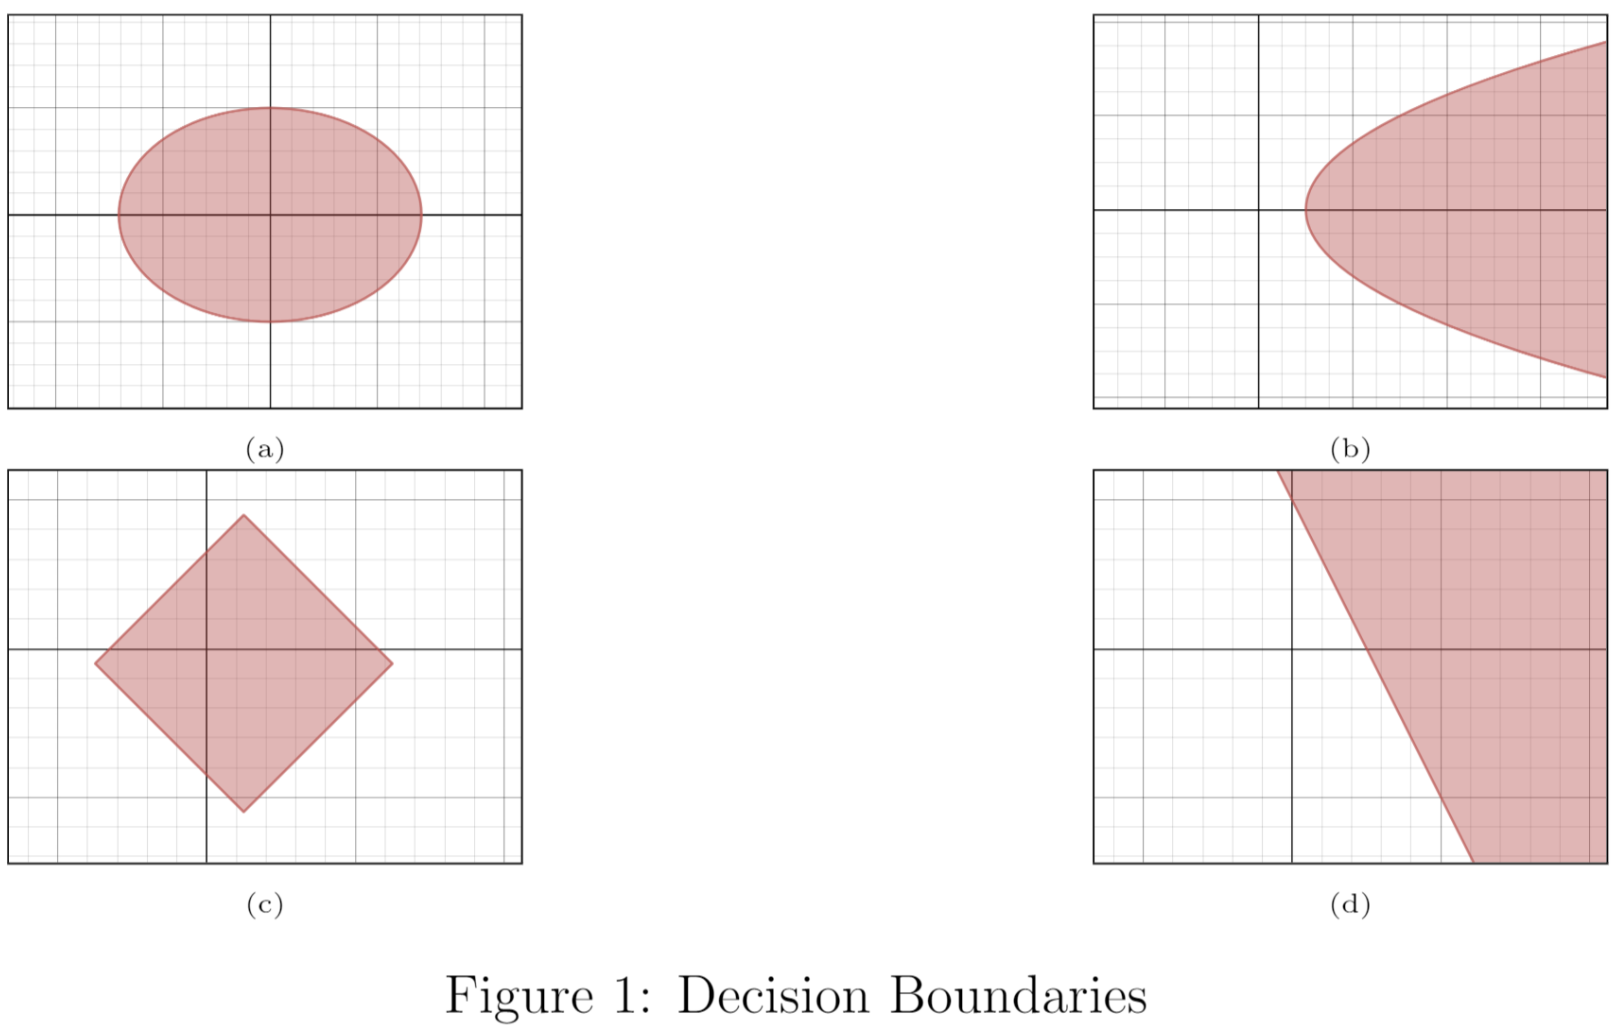
\includegraphics[scale=0.43]{figs/GNB_decision_boundary.png}
    \end{figure}
    {\checkboxchar{$\Box$} \checkedchar{$\blacksquare$}
    \begin{checkboxes}
        % YOUR ANSWER 
        \choice (a)
        \choice (b)
        \choice (c)
        \choice (d)
        \choice None of the above
    \end{checkboxes}
    }
    

    \newpage


    
    \part Suppose we want to extend the Naïve Bayes model to time series data. Formally, a training data point consists of a binary label Y and D sequentially ordered observations of a binary outcome where $X_1$ occurs before $X_2$, which occurs before $X_3$ and so on all the way down to the final observation $X_D$; each feature $X_d$ is binary. \\

    You decide to modify the Naïve Bayes assumption such that a feature $X_d$ is conditionally independent of all other features given the label Y and the previous feature $X_{d-1}$; the first feature $X_1$ is conditionally independent of all other features given just the label Y. The corresponding Generative story would be: 
    \begin{align*}
    Y &\sim \text{Bernoulli}(\phi) \\
    X_1|Y &\sim \text{Bernoulli}(\theta_{1,y})\\
    X_d | X_{d-1},Y & \sim \text{Bernoulli}(\theta_{d,x,y})
    \end{align*}
    where the parameters are the Bernoulli parameter $\phi$ and, the class-conditional Bernoulli parameter $\theta_1$ , and the class-conditional Bernoulli parameters $\theta_{d,x,y}$ for $X_d | X_{d-1} = x, Y = y$. 

    \begin{subparts}
        \subpart[2] Write down the expression for the joint distribution $P(X,Y)$ under your new Naïve Bayes model. You don't need to plug in the values of the pdf, you can leave it as probability expressions. You must use the modified Naïve Bayes assumption described above \\
        \begin{your_solution}[height=3cm]
        % YOUR ANSWER 
    
        \end{your_solution}
        

        \subpart[1] How many parameters do you need to learn in order to make predictions using this new Naïve Bayes model? Write your answer in terms of D.\\
        \begin{your_solution}[width = 4cm,height=2cm]
        % YOUR ANSWER 
    
        \end{your_solution}
        

        \subpart[2] Suppose we train this model via MLE. In at most 2 sentences, 
        describe how we would estimate $\phi$\\
        \begin{your_solution}[height=3cm]
        % YOUR ANSWER 
    
        \end{your_solution}


        \subpart[2] In at most 2 sentences, describe how we would estimate $\theta_{d,x,y}$ for $2 \leq d \leq D$ using MLE.\\

        \begin{your_solution}[height=3cm]
        % YOUR ANSWER 
    
        \end{your_solution}


        

        
    \end{subparts}
    

 
    
    
    % \part[2] \sall Neural the Narwhal used a 2D Gaussian Naïve Bayes model for a binary classification task, and obtained the following contour plot for the density $f(x_1, x_2 \mid y=+)$. You instantly notice that he made a mistake. Why is his result theoretically impossible to be obtained from a Gaussian Naïve Bayes model?
    % \begin{center}
    %     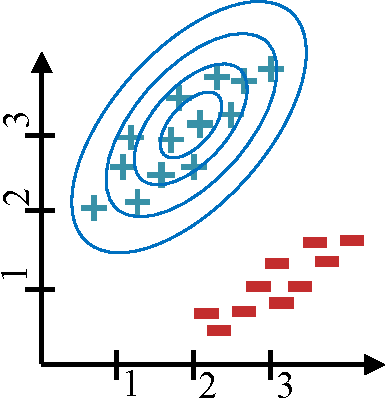
\includegraphics[width=4cm]{figs/contour.pdf}
    % \end{center}
    % {\checkboxchar{$\Box$} \checkedchar{$\blacksquare$}
    % \begin{checkboxes}
    %     % YOUR ANSWER 
    %     \choice The mean of the distribution should be the mean of all points, not just positive points ($+$)
    %     \choice A Bernoulli Naïve Bayes model should be used instead for discrete labels ($+$ and $-$)
    %     \choice The covariance matrix of the distribution is not a diagonal matrix
    %     \choice None of the above
    % \end{checkboxes}
    % }
    

    
\end{parts}\newpage
\sectionquestion{Generative vs. Discriminative Models}

\begin{parts}

\part[2] \sall
Which of the following models are discriminative?
{\checkboxchar{$\Box$} \checkedchar{$\blacksquare$}
\begin{checkboxes}
    % YOUR ANSWER 
    \choice Logistic Regression with L2 regularization 
    \choice Logisitic Regression without L2 regularization
    \choice Naive Bayes
    \choice KNN
    \choice Decision Trees
    \choice None of the above
\end{checkboxes}}


% \part[2] \textbf{True or False: } Discriminative models work better with unlabelled data.
% \begin{checkboxes}
%     \choice True
%     \choice False
% \end{checkboxes}


% \part Consider the cases where we have outliers in our training data.
% \begin{subparts}

% \subpart[1] {} \textbf{True or False: } Generative models tend to be more heavily affected by outliers.
% \begin{checkboxes}
%     \choice True
%     \choice False
% \end{checkboxes}

% \subpart[2]{} Explain your answer in 1-2 sentences.

% \begin{your_solution}[height=3cm]
% % YOUR ANSWER 

% \end{your_solution}
% \end{subparts}
\part Consider the following dataset $D$ for 1D Logistic Regression and Gaussian Naive Bayes. There are nine points with label $y=1$ at $x=1$, one point with label $y=1$ at $x=2$, nine points with label $y=0$ at $x=-1$, one point with label $y=0$ at $x=-2$. In addition, we have another dataset $D'$, which is an exact duplicate of $D$, except in addition, we have two outliers, one point with label $y=0$ at $x=10$, and one point with label $y=1$ at $x=-2$. For the following questions, \textbf{round your answer to 3 decimal places.}

\begin{subparts}
\subpart[1] What is the decision rule for Logistic Regression on $D$? In other words, find the $C$ such that Logistic Regression will predict $y=1$ for $x \ge C$.

\begin{your_solution}[width = 4cm,height=2cm]
    %YOUR ANSWER
\end{your_solution}


\subpart[1] What is the decision rule for Naive Bayes on $D$? 

\begin{your_solution}[width = 4cm,height=2cm]
    %YOUR ANSWER
\end{your_solution}


\subpart[1] We ran logistic regression on $D'$, and learned that the bias term is $\beta_0 = -0.0515$, and the weight is $\beta_1 = 0.1859$. What is the decision rule for this dataset (with the outliers)?

\begin{your_solution}[width = 4cm,height=2cm]
    %YOUR ANSWER
\end{your_solution}

\newpage

\subpart[5] What are the parameters for our Gaussian Naive Bayes classifier on $D'$, if we train via MLE? 

\begin{subparts}
    \subpart $P(Y=1)$
    \subpart mean for $P(X|Y=1)$
    \subpart variance for $P(X|Y=1)$
    \subpart mean for $P(X|Y=0)$
    \subpart variance for $P(X|Y=0)$
\end{subparts}

\begin{your_solution}[width=4cm,height=2cm, title = (a)]
    %YOUR ANSWER
\end{your_solution}
\begin{your_solution}[width=4cm,height=2cm, title = (b)]
    %YOUR ANSWER
\end{your_solution}
\begin{your_solution}[width=4cm,height=2cm, title = (c)]
    %YOUR ANSWER
\end{your_solution}
\begin{your_solution}[width=4cm,height=2cm, title = (d)]
    %YOUR ANSWER
\end{your_solution}
\begin{your_solution}[width=4cm,height=2cm, title = (e)]
    %YOUR ANSWER
\end{your_solution}


\subpart[2] What is the new decision rule for Naive Bayes on $D'$? Note you might get two numbers, since the decision rule is a bounded interval. Please find $C_1$ and $C_2$ such that Naive Bayes will predict $y=1$ for $C_1 \le x \le C_2$.

\begin{your_solution}[width = 4cm, height=2cm]
    %YOUR SOLUTION
\end{your_solution}


\subpart[3] Based on your answers to the previous questions, which one of Logisitic Regression and Naive Bayes is more resistant to outliers? Compare the decision boundaries on $D$ and $D'$ for Logistic Regression and Naive Bayes. Explain your reasoning in 2-3 sentences. 

\begin{your_solution}[height=3cm]
    %YOUR SOLUTION
\end{your_solution}


\end{subparts}

\newpage

% \part[2] Assume that the dotted line represents the error vs. number of examples for Logistic Regression, and the solid line is for Naive Bayes. Observe that for around $m \ge 15$, where $m$ is the number of examples in the training dataset, Logistic Regression yields a lower error than Naive Bayes. Explain why this may be the case, based on your understanding of generative vs. discriminative models. 
% \begin{center}
%     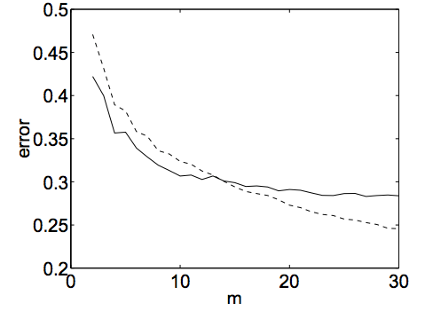
\includegraphics[scale=1.5]{hw6/figs/LRvsNB.jpg}
% \end{center}


% \begin{your_solution}[height=3cm]
%     %YOUR SOLUTION
% \end{your_solution}


\end{parts}\newpage
\sectionquestion{Google Colab}

Please refer to the notebook \href{https://colab.research.google.com/drive/1Pe8rjLHKRT-zjjzvBXNPeR0KgoglQFDD?usp=sharing}{here} as well as the google colab setup \href{https://scs.hosted.panopto.com/Panopto/Pages/Viewer.aspx?id=8d010cf2-9358-4a44-a11e-b0a601007803}{video} for the following questions. \textbf{Please upload a screenshot of the commands being run and the outputs}, so that we can verify that you have successfully setup google colab for the next homework. When running the commands below, make sure that you are connected to a GPU.
\begin{parts}
    \part[1] Upload a screenshot of the output of mounting your drive onto your notebook. On the left hand side, please show the folders in your drive(It is ok to just show the MyDrive folder, we just need to see it). In your screenshot, also include that you are connected to a GPU, which you will see on the right hand side of the page. 
    
    \begin{your_solution}[height = 8cm]
        %Upload a screenshot of the command and the output
        
    \end{your_solution}
    
    \part[1] Upload a screenshot of running the following commands:
        \texttt{torch.cuda.is\_available()}, \texttt{torch.cuda.device\_count()}, and \texttt{torch.cuda.get\_device\_name(0)}.\\
    \begin{your_solution}[height = 8cm]
        %Upload a screenshot of the command and the output
        
    \end{your_solution}
\end{parts}\newpage
\newpage
\section{Collaboration Questions}
After you have completed all other components of this assignment, report your answers to these questions regarding the collaboration policy. Details of the policy can be found \href{http://www.cs.cmu.edu/~mgormley/courses/10601/syllabus.html}{here}.
\begin{enumerate}
    \item Did you receive any help whatsoever from anyone in solving this assignment? If so, include full details.
    \item Did you give any help whatsoever to anyone in solving this assignment? If so, include full details.
    \item Did you find or come across code that implements any part of this assignment? If so, include full details.
\end{enumerate}

\begin{your_solution}[height=6cm]
% YOUR ANSWER 

\end{your_solution}
\end{questions}


\end{document}